% This is samplepaper.tex, a sample chapter demonstrating the
% LLNCS macro package for Springer Computer Science proceedings;
% Version 2.20 of 2017/10/04
%
\documentclass{llncs}
%
\usepackage{graphicx}

\begin{document}
% Adicionado para por apenas os numeros sem headers
\pagestyle{myheadings}
\title{Development of text-mining solutions to facilitate lipid metabolism interpretation in Genome-Scale Metabolic Models}

\author{Adriano Silva\inst{1}\and
João Ribeiro\inst{1}\and
Emanuel Cunha\inst{1}}

\institute{University of Minho}
%
\maketitle              % typeset the header of the contribution
%
\begin{abstract}
Systems Biology is gaining importance in the unveil of cellular secrets. More precisely GSM models allow the contextualization of omic data and the progress of genomic engineering.
Still, the lack of macromolecule structural defined representation, such as lipids, is glaring.

-- Generic and defined duality

-- Resolution

\keywords{Genome-Scale Metabolic Models  \and Lipids.}
\end{abstract}
%
%
%
\section{Introduction}
\subsection{Context and motivation}
In the past two decades, Systems Biology has emerged as a discipline capable of integrating molecular biological knowledge into an understanding at a system level, from a complete, precise, and efficient perspective.
Biological systems represent a huge amount of data, with the need to be treated and contextualized where this discipline comes to the aid.  
Whether in the construction of stochiometric models or the reconstruction of genome scale metabolic models (GSM), with means to understand the genomic, biochemical, and physiological knowledge gathered \cite{Zou2018,Tavassoly2018}. 
These approaches can guide to strain optimization and the production of a compound with industrial interest, such as lipidic biofuel produced by optimized yeasts and microalgae \cite{Sawangkeaw2013}.

Impulsed by the advances and cost-effectiveness in technologies that led to high-throughput biological data (Big Data), Systems Biology, and more precisely the reconstruction of GSM models is gaining importance.
The reconstruction of GSM models is taking advantage of the high-quality data generated to create better simulations and predictions. 
In total, since the reconstruction of the first GSM model in 1999 \cite{Edwards1999}, 6239 GSM models were reconstructed until 2019 \cite{Gu2019}. 
Nonetheless, the pace of reconstruction of GSM models can't keep up with the growth of Big Data. The lack of integration of new data in GSM models is a problem inherent to this growth discrepancy.

Besides the usefulness of these models, their reconstruction is limited due to the lack of biochemical and structural data incorporated.
Complex macromolecules are often represented in their generic version not giving any biochemical and structural information \cite{Gu2019}.
Particularly in the case of lipids, only a small chunk of GSM models reconstructed have structurally defined lipids. 
These models neglect the fact that each class is constituted of a countless number of combinations between the different components of the lipid. 
Thus the GSM models in these conditions are not able to capture the integrity of the lipid biosynthesis network.
Therefore it is important the integration of such information into lipidic models, for better interpretability, handling, and predictions.

Integration of the structural information can be done by taking advantage of the  \emph{de facto} tools such as SWISS LIPIDS \cite{Aimo2015} and  LIPID MAPS \cite{Sud2007}.
As mentioned above this is important to the reliability of the model allowing credible predictions and flexibility in the management of the model.
This can turn into a major advancement in lipid models with better application in industry, such as in the case of lipidic biofuels \cite{Sawangkeaw2013}.




\subsection{Objective}

The main objective of this project is to integrate lipidic structural data, from \emph{de facto} tools SWISS LIPIDS and LIPID MAPS, into a graph-based database BOIMMG.
It will be done through the integration of the synonyms and abbreviations into a new label using ETL pipelines. 

\section{State of art}
\subsection{Genome Scale Metabolic Models}
The use of computational tools brings to the science new tools to face the challenges in the scientific scope.
Among them are GSM models, a computational tool that conjugate biochemical and genomic data from an organism, with the capacity to do \emph{in silico} predictions of a given organism phenotype in specific environmental and genetic conditions \cite{Rocha2007,Zhou2021}.

Thus, these models are key to the contextualization of high throughput data and helpful in many other applications such as metabolic engineering, production of biochemicals and bio-materials, prediction of enzyme functions, or even in the discovery of drug targets\cite{Gu2019,Kim2017}.
It is therefore important to integrate fresh and reliable biochemical data in the reconstruction of these models to ensure their accuracy and further actualization \cite{Moseley2021,Passi2021}. 


\subsection{Lipid computational representation}
Lipids are a unique macromolecule grouped into different classes accordingly to their structural composition. They are composed by two distinct components, distinction in their composition confers to lipids the characteristic of amphipathic molecules. 
This characteristic allows the generation of micelles in a hydrophilic environment, which is important for their biological roles such as being the principal cell membrane components, energy storage, and signaling molecules.

Structurally it is impossible to say how many distinct lipids are due to the multitude of arrangements that can make a different structure \cite{Gyamfi2018}. 
The definition of the lipid class is well-established, existing already eight main classes defined \cite{Fahy2011}.
Lipid structure can be split into two different parts the backbone, and the side chain represented in Fig.~\ref{fig1}. The first one gives the lipid the name of the class, remaining the same to the whole lipids in the same class.
In the case of side chains, their structure can vary in the same class both in the number of double bonds and in the identity of the chains, giving rise to new subclasses.

\begin{figure}
    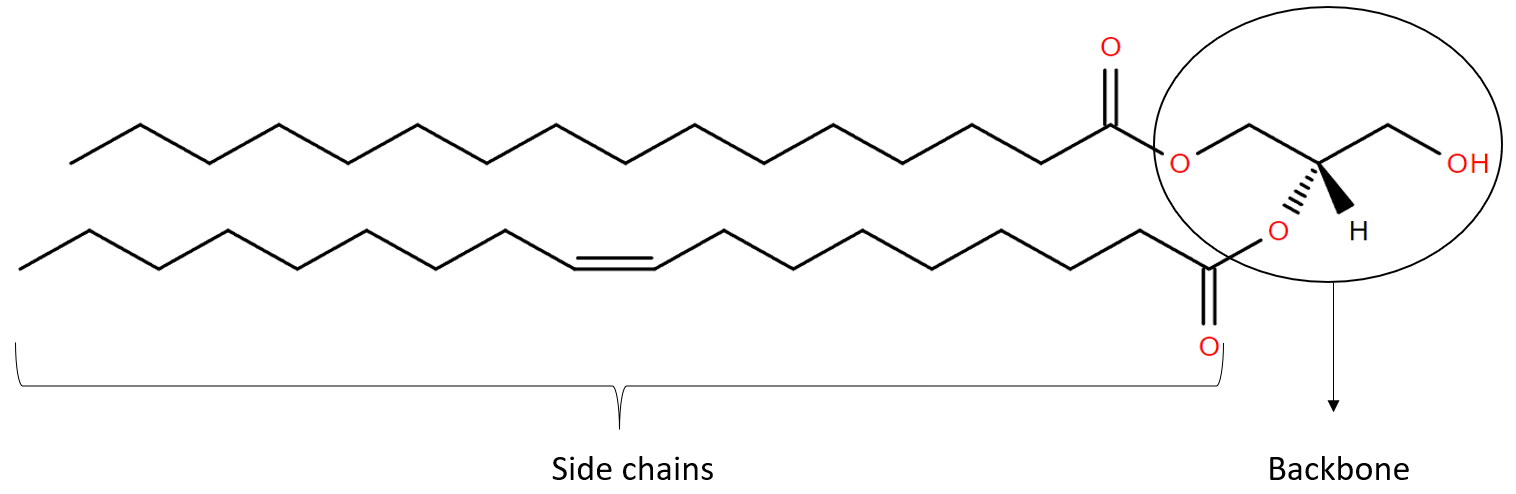
\includegraphics[width=\textwidth]{imagens/lipido.png}
    \caption{Representation of 1-hexadecanoyl-2-(9Z-octadecenoyl)-sn-glycerol structure extracted from LIPID MAPS.The backbone is the hydrophilic part of the lipid while the side chains confer hydrophobicity.} \label{fig1}
\end{figure}

The grown importance of this macromolecule in health research and industrial applications brings more than ever the need to characterize their metabolic network and roles in cells.
Due to the immense amount of reactions, and complex biosynthetic pathways where lipids play a role, it is almost impossible to study them in classical means \cite{Schutzhold}.

Computational approaches are helping to disentangle these complications however, lipid representation is not always well implemented.
Despite the existence of lipid databases with defined structures, computational representation is often done generically \cite{Aung2013}. 
This means that the representation in computational approaches is only given by the backbone name, remaining the side chains as simple R groups.
Given the importance of the structure in metabolic interactions, this hides information not allowing to achieve the full potential of these approaches.

\subsection{Generic Representation in GSM models}
To reduce the complexity of the implementation, due to lipidic complex structures and their high variability, lipid representation on GSM models is often generic (figura com a representação generica de um modelo?). This representation neglects the fact that side chains are important components in the lipid metabolic network \cite{Fahy2011,Schutzhold}.

Accordingly, biosynthetic pathways are represented in generic terms, with generic lipids as reactants and products.
Based on this, we cannot access the specific lipid used in an hypothetic biosynthetic network due to the number of lipids represented with the same backbone name.
Besides that, an abstract representation is linked to the loss of specificity of individual reactions, the use of lipidic species that should not be present in the model, and to the impossibility to reach a defined structure through a generic one.\cite{Aung2013}.

The capacity to interchange side chains and form new lipids, with probable new metabolic interactions, turns this type of representation not helpful in acknowledging the lipidic metabolic network.
Interestingly, we can still see the presence of cross-references to databases with the structure of these macromolecules. However, the same structure serves many lipids due to its abstract name.

\subsection{Structurally defined representation in GSM models}
Contrary to the generic representation, seeing defined ones in GSM models is not usual and only a few chunks of the reconstructed GSM models have lipids structurally defined \cite{Schutzhold}.
Here is also defined the constitution of the side chains as a second part of the lipid structure name. This is done using the number of carbons in the chain followed by the number and the location of double bonds as well as their conformation for each side chain (figura a demonstrar esta representação??).

This approaches allows the generation of individual reactions with structurally defined lipids, oppositely to the whole species of lipids used in the generic representation \cite{Aung2013}.
GSM models with defined lipids are more reliable,  allowing the improvement of the flexibility, accuracy, and level of detail in these models.
Besides that, we can witness a lack of references, which is not ideal for lipid structural confirmation.

\subsection{Lack in lipid annotation in GSM models}
primeiro paragrafo

- Merge the two previous logics (sucintamente)
- falar das anotações, uma tem e outra tem poucas.

Segundo

- Possível Resolução
    - integração dos sinonimos e abreviaturas das bases de dados xyz com ETL
    uma frase para cada e um paragrafo para etl ( esquema pode ajudar??)

Terceiro?   

Anotação de modelos:
    - match direto
    - decomposição do nome em dois (backbone e side chain) - queries à base de dados
\begin{figure}
    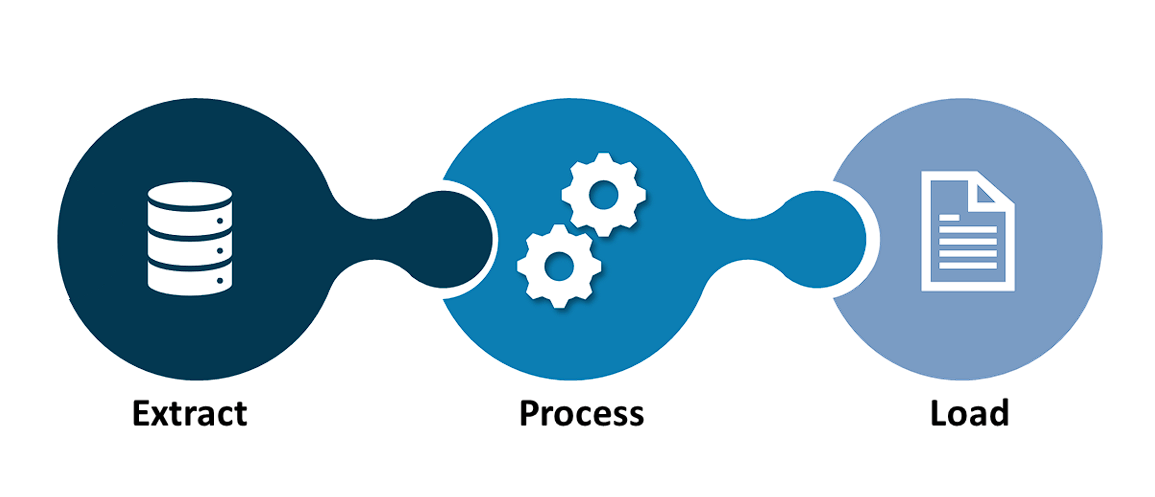
\includegraphics[width=\textwidth]{imagens/ETL.png}
    \caption{Escheme of the process done with ETL pipeline.
    First gather data from conventional databases
    then processes that data
    and finally integrates the data in our database.} \label{fig2}    
\end{figure}





\bibliographystyle{ieeetr}
\bibliography{referencias.bib}
\end{document}
